\section{Methodology, ethics, and repeatability of case studies} \label{section-methodology-ethics-and-repeatability-of-case-studies}

\begin{figure}
    \centering
    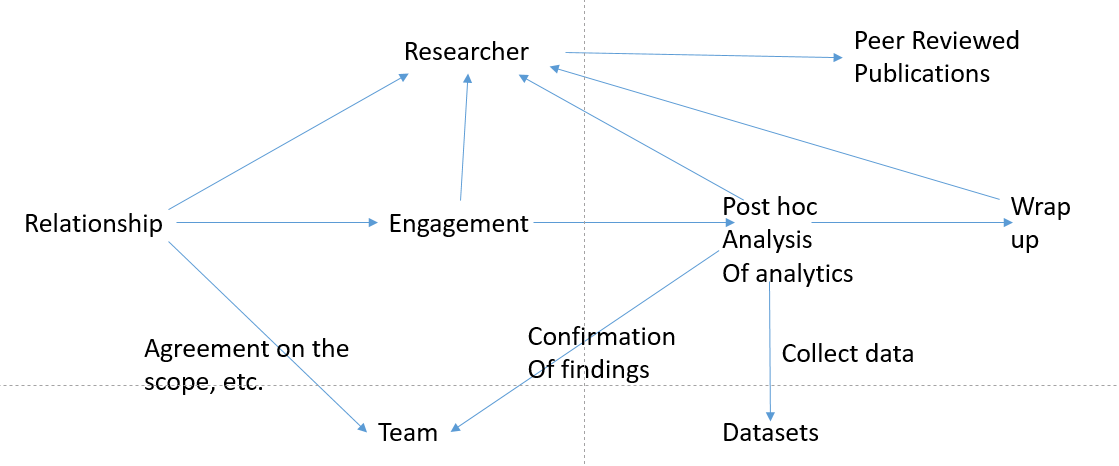
\includegraphics[width=14cm]{images/rough-sketches/Yijun-rough-sketch-of-relationships-in-case-study-methodology.png}
    \caption{Yijun's rough sketch of the methodology- a w-i-p}
    \label{fig:yijun-methodology-sketch}
\end{figure}

\subsection{Methodology}
The methodology needs to address the phases of each case study that involves projects and their respective organisation; namely: exploration and selection, engagement, the active case study (including data collection, contemporary analysis, and any contributions to the project), \emph{post-hoc} analysis and verification, wrap-up, and publication. These phases may overlap somewhat, they are in approximate time order from first to last. They are covered in order below.

\subsubsection{Exploration and selection}
\begin{wrapfigure}{R}{0.5\textwidth}
  \begin{center}
    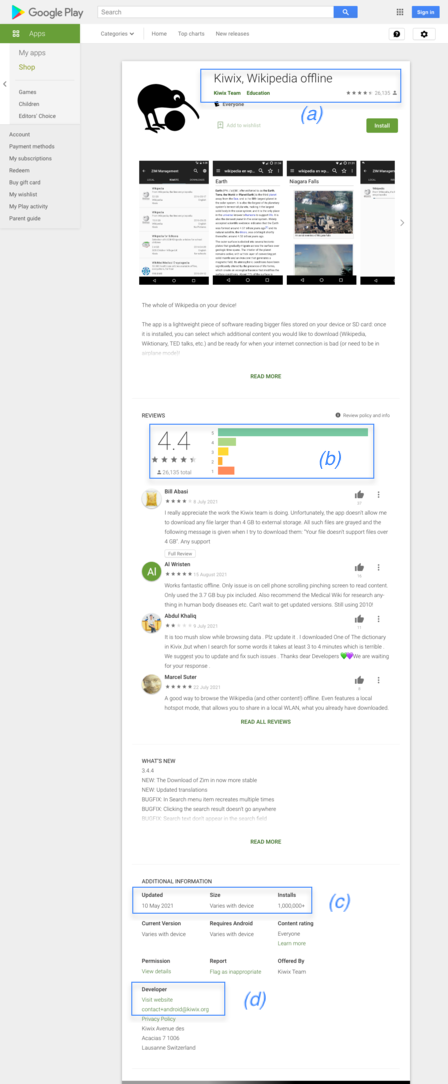
\includegraphics[width=0.42\textwidth]{images/google-play/annotated-resized40pct-2021-09-30-kiwix-app-on-google.png}
  \end{center}
  \caption{Kiwix: app presented in Google Play Store}
  \label{fig:gp-kiwix-app}
\end{wrapfigure}

The projects and their respective organisation need to develop mobile apps and be willing to have mobile analytics for their apps. For the case studies in this research every project included at least one actively used Android app in Google Play\footnote{By having an active app in Google Play they will also have access to the Google Play Console with its dashboard, Android Vitals, release tools, and other related reports. Therefore they will \emph{de-facto} have at least one source of analytics, collected by the Google Android platform.}, however the methodology may work with minor variations for other app stores and mobile platforms.


Various forms of exploration are available. For apps in major app stores the app store may provide pertinent information that can be used to preliminarily select target apps. Figure~\ref{fig:gp-kiwix-app} is how the Kiwix Android app appears to visitors to Google Play when using a web browser (Firefox in this example). Four areas of pertinent information have been highlighted:

\begin{enumerate}[label=(\alph*)]
    \itemsep0em
    \item The category of the app and the count of ratings. The category helps group case studies by category, and also helps compare a particular app with the median crash and ANR rates for apps in that category. More details on these are available in \secref{section-peer-categories}.
    \item More details of the distribution of the ratings.
    \item When the app was last updated in the app store and the number of installs of all versions of this app.
    \item Contact details for the developer~\footnote{That said, like many relationships, a warm lead is more likely to elicit a response than a cold email to the published email address. For this research all bar one of the case studies was established through a warm lead, someone who knows me. The exception was the \href{https://github.com/Phantast/smartnavi}{Smartnavi} project where the connection was established through email.}.
\end{enumerate}


\subsubsection{Engagement}
The engagement phase includes discussions to determine whether the project team (and their organisation) and the researcher(s) would be willing to participate in a viable and productive case study. It is also a suitable time to agree on the depth, scope, range, and duration of the case study. Similarly concerns and constraints need to be determined and agreed that protect all the stakeholders involved while also allowing the research to be not deliberately biased by the project team/organisation. The stakeholders may extend beyond the primary participants, for instance the end users could potentially be stakeholders in what happens during the case study.

There may also need to be discussion, joint understanding, and agreement on: intellectual property rights, copyright, confidentiality, non disclosure agreements, and so on~\footnote{Note: some researchers may be introduced to these together with the ethical aspects under the term LSEPI, discussed in ~\citet{brooke2018__becoming_professional_a_university_perspective}}. Researchers may be subject to their contract with their institution, employer, and so on. The project team and organisation sometimes may be concerned about any intellectual claims by the researcher's organisation. For the research covered in this thesis copyright is retained by the researcher.

As \citet[p.324]{barroca_2018_bridging_the_gap} notes timeliness and relevance are vital to industry partners, while they also want to guard against the research being too intrusive or too demanding of their time or other resources. Therefore the research needs to offer something of sufficient relevance and timeliness to the project team and their organisation. 

The ROI of empirical research was discussed and published a relatively long time ago from the perspective of scientific and industrial views~\citet[pp54-57]{prechelt_2007_optimizing_ROI_for_empirical_SE_studies}. Investment in case studies includes dealing with the researcher and their demands so if the researcher is able to use mobile analytics tools, analyse the reports, and investigate initial findings they may reduce the burden placed on the project team and their organisation.

Fortunately research into using mobile analytics to improve the quality of their mobile apps has often provided relevant and timely contributions to the projects, particularly in the more in-depth case studies. Also the projects generally already have at least one form of mobile analytics so the incremental cost is low in terms of tooling.
 
\subsubsection{The active case study}
If the researcher has direct access to the mobile analytics and/or other materials (such as source code, issue tracking) they can perform at least some of the research directly. If the engagement also includes contributions to the project's materials similarly the researcher may be able to contribute directly if they have write access and/or the facility to fork the codebase and create pull requests. Otherwise the route to mobile analytics reports and any other material available is indirect, via someone who is part of the project and collaborating in the case study. All the case studies included elements of working with and through at least one member of the project team.

For the in-depth case studies where the researcher is more actively involved with the project, the research is likely to have opportunities to work with a variety of team members, and they are also more likely to have direct access to mobile analytics and at least some of the resources. Notes made during and immediately after interviews help to record what was discussed, together with any agreements, actions, or outcomes pertinent to the research and/or the project. Subsequent checking and confirmation of the discussion, for instance in a summary email to the other people in the discussion, 

\citet[p.250]{falessi2010_applying_ESE_to_sw_architecture_etc} states \emph{``there is now a growing need to systematically gather empirical evidence about the advantages or otherwise of tools and methods rather than just rely on promotional anecdotes or rhetoric."}. That was published in 2010, similarly in current times over a decade later, there is a similar growing need to gather evidence about the use of mobile analytics.

In terms of the methodology, during the active case study it is vital to collect and perform ongoing analysis of mobile analytics and whatever other materials are available. Many of these are ephemeral in nature. for instance graphs may change by the minute.  Third-party mobile analytics (including those provided by Google) have terms of use. These terms of use have various names, such as a policy, \textit{e.g.} for Google Play ~\citet{google_play_developer_policy_center}. These may place limitations on data collection and use of the relevant service. For the research covered in this thesis a conservative approach was used in terms of data collection to reduce the risk of consequential issues for the researcher, the project, and the stakeholders for the app. This topic and the implications are expanded on in the \secref{chapter-discussion} chapter.

The choice of tools, including the humble web browser used by the researcher, affects aspects of the ease of collection of on line reports. As an example, the screenshot capability of the Mozilla Firefox browser~\footnote{Described in \url{https://screenshots.firefox.com/}} is far richer than that provided by Google Chrome at the time of writing. Many of the reports in mobile analytics tools require extensive vertical scrolling, Firefox can capture the entire contents easily, Chrome does not. 

Similarly some content is only generated on screen on demand, in response to user actions, for example through scrolling vertically and/or paging through reports. Therefore, to capture the content the researcher (or their human/automated proxy) needs to perform these actions to obtain these contents and pertinent materials saved/safeguarded to facilitate longer term analysis and provide/record evidence. Note: it is not always practical or useful to record ``everything"; how much is suitable is a topic for future research. Where practical aim to collect the underlying text in addition to visual content; the text can then be processed relatively easily and without needing to be re-keyed.

\subsubsection{\emph{Post-hoc} analysis and verification}
By this stage, the active case study has finished, in some cases additional updates may be available, for instance if there is ongoing access to mobile analytics as some projects have provided in this research and/or updates from the project team. Nonetheless, for the most part the evidence has been harvested and any active interventions have ceased. The time has come to perform \emph{post-hoc} analysis and verify the findings and analysis with the project team. 

One objective is to make the \emph{post-hoc} analysis repeatable, where others can perform the analysis and obtain similar results; therefore this section explains various patterns of analysis and there are various worked examples provided in the individual case studies.

\begin{itemize}
    \item Collating similar failures:
    \item Bug identification and localisation: Establishing potentially pertinent patterns in the reports.
    \item Ordering and ranking clusters of failures:
    \item Bug investigation:
    \item The triage process: 
    \item Comparing information sources:
    \item ...
\end{itemize}

% X-ref to the six perspectives and the findings. What are the data sources that helped me understand the 3 status quo's and the 3 areas or improvement.
In Figure~\ref{fig:six-perspectives} six perspectives are illustrated; these perspectives may help to categorise and group various findings in the \textit{post-hoc} analysis. 



\subsubsection{wrap-up}

\subsubsection{publication}
\isabel{publishing for industry AND for academia}


\textbf{TODO expand on these points}
\begin{itemize}
    \item Notes made during and immediately after interviews... Subsequent checking and confirmation of what was agreed
    \item Caveats for those who follow...
    \item Notes to self :)
    \item ...
\end{itemize}

\subsubsection{Establishing patterns of case studies}
\julian{c.f. blood group types O positive, o negative, etc.}



\subsection{Repeatability}
\textbf{Expand on:} What's hard to repeat (and why), aims to improve and demonstrate repeatability of the practices applied in this research.

\isabel{suggests repeatability is part of good research ethics.}
\isabel{Research as a political statement c.f. her transfer report.}

\begin{comment}
TODO papers to consider discussing here include: 
\begin{itemize}
    \item ``R3: repeatability, reproducibility and rigor"~\citep{vivek2012_r3_repeatability_reproducibility_and_rigor}

\end{itemize}
\end{comment}


\subsection{Research ethics for the case studies}
\label{section-research-ethics-for-the-case-studies}
The majority of the case studies presented in this research include other people. It is right and proper to ensure they and their respective organisations are willing to support the research directly - by participating - and/or indirectly - for instance by providing access to systems, tools, bug tracking systems, and so on. Some organisations require non disclosure agreements, and - in practice - they all choose what access to provide to what, to whom, and for how long. 

Engagement and trust need to be established with the people who manage the project and with the people who participate in the case study. Organisations often require approval from one or more senior representatives in the organisation, these may include head of development, and one or more of their legal, marketing, commercial, and risk departments.

For startups, one person may hold multiple roles, for instance in small startup teams they may be the CTO while also being an active developer of the software, \emph{and} the person responsible for operations, support and customer service. This was the case for two of the case studies presented in this research (LocalHalo and Iteratively), and in Moodspace the CTO was also the main developer of the app. In terms of obtaining permission, startups tend to be easy to work with if they agree to support the research as one or two people can quickly decide to support the research and provide access to whatever materials they are willing to share. They may not have time or patience to read or sign formal agreements, however an email summary of any verbal agreement helps to sum up that agreement and provide them the opportunity to confirm, clarify, or reject the contents of the agreement.

Mutualism, commensalism, parasitism, predation and competition are five types of symbiotic relationship. % ``There are five main symbiotic relationships: mutualism, commensalism, predation, parasitism, and competition."  Symbiosis: The Art of Living Together https://www.nationalgeographic.org/article/symbiosis-art-living-together/ 
Of these the last three may produce adverse outcomes for at least one participant.
In computer science research that involves organisations and live projects the type or types of symbiotic relationship(s) are another key consideration. The candidate projects and their organisations need to be confident that if they participate as case studies in research that they will not suffer in the relationship. If they see mutual benefits of the research they may be more willing to actively participate. 

As \citet[p.2]{robinson2019_applying_endosymbiosis_theory_tourism_and_its_young_workers} observe: \emph{``Business, or work, ecosystems are a community of interacting organisations and individuals (or groups) – or the organisms of the commercial world"}. Their research was into the relationships of Tourism and its young workers, and the possibility for exploitation in either or both directions. The challenges in their domain may apply to this type of case study based research and the researcher is wise to consider the potential adverse effects for any of the parties involved in the case study.

Another consideration is the concept of `agency' that the organisations and the relevant people are free to choose whether they wished to participate in the research. Some candidates declined to participate in the research on behalf of their project or organisation for various reasons. A common reason was lack of time on their part, another was that some candidates perceived the research would not be acceptable to their organisation, for instance owing to confidentiality or business risk.

The participants choose their model of engagement, this means the research needs to be adapted to their engagement model, availability, and ways of working. The researcher may need to bridge between and/or mediate between the academic research ways of working and those practiced in industry, and here in the domain of mobile app development. In particular the researcher needs to uphold the expectations of both academia and industry, this may be easier for someone who has sufficient experience and competence in both ecosysystems.

\newthought{How were these research concepts applied in this research?}
Every one of the actual case studies, and those that did not come to pass, started with a connection between two or more people. Sometimes the connection was indirect via someone who knew of the research. In several cases the relationship was established by someone at the candidate case study who was aware of the researcher and the research. There will be other ways to recruit potential case studies, however they were not used for this research.

However an initial contact/communication came about thumbnail of the research was presented to the candidate. This included an explanation that at least some of the work would need to be permitted to be published as part of the research and that permission would need to be freely given. With the exception of a particular commercial case study the engagement was voluntary and unpaid. The particular commercial case study ran alongside a paid consultancy where the researcher was engaged to help address challenges in one or more projects with similar aims to this research. Details of the organisation, the project(s), and the particular results are constrained by a commercial non-disclosure agreement.

For the two direct engagement case studies for opensource projects, they both asked for help to improve the reliability of at least one of their Android apps. Therefore the engagement had the potential to be mutually beneficial. Similarly, for the case studies with mobile analytics tool/service providers they saw value in being engaged with the research and the immediate results of those case studies. For the developer interviews the symbiotic relationship was closest to being commensal, while they may glean some benefits, it was not a primary factor in their willingness to participate. Instead they were keen and willing to help with the research for the good of the research. 



\begin{itemize}
    \item Ethics review for Workshop in Poland (and then for various reasons the contents of the workshop were not viable because of the effects of COVID-19.
    \item No other human subjects, the data related to apps and how the app is used and performs, humans are not the subject of the research.
    \item Opensource, freely available apps without any restrictions on sharing the findings of the performance of the apps. No PII information collected by the analytics tools used.
    \item Semi-structured interviews with various individuals in their professional and/or project capacities.
\end{itemize}

Participants were briefed and gave their permission either individually or on behalf of their organisations to use the material they freely provided. Several have reviewed my research and provided constructive feedback which has been applied. 
It has not always been practical to reach them, for instance some are no longer reachable. None of the analytics information provided contains PII.

Some of the opensource projects that form part of this research received and accepted pull requests from the researcher, these were freely given and freely received and have no known monetary value.

\begin{comment}
TODO papers to consider discussing in the ethics section include: 
\begin{itemize}
    \item ``The human is the loop: new directions for visual analytics"~\citep{endert2014_the_human_in_the_loop_new_directions_for_visual_analytics}
    \item ``Not All Trust Is Created Equal: Dispositional and History-Based Trust in Human-Automation Interactions"~\citep{merritt2008_not_all_trust_is_created_equal_etc}.
    \item \emph{``Symbiosis
Symbiosis refers to the partnership (usually long-term) that is established between two or more organisms. In microbiology, symbiotic relationships are often established between a microorganism and its host, and the partnership can be mutualistic or parasitic."} \url{https://www.nature.com/subjects/symbiosis}
\end{itemize}
\end{comment}

\clearpage